% ------------------------------------------------------------------------------
% FORMATVORLAGE DOKU/ BEDIENUNGSANLEITUNG
% ------------------------------------------------------------------------------

% DOKUMENTENKOPF ---------------------------------------------------------------
%   Diese Vorlage basiert auf "scrreprt" aus dem koma-script.
% ------------------------------------------------------------------------------
\documentclass[
    11pt,    % Schriftgr��e
    DIV10,
    ngerman, % f�r Umlaute, Silbentrennung etc.
    textgreek,
    a4paper, % Papierformat
    oneside, % einseitiges Dokument
    titlepage, % es wird eine Titelseite verwendet
    parskip=half, % Abstand zwischen Abs�tzen (halbe Zeile)
    headings=normal, % Gr��e der �berschriften verkleinern
    listof=totoc, % Verzeichnisse im Inhaltsverzeichnis auff�hren
    bibliography=totoc, % Literaturverzeichnis im Inhaltsverzeichnis auff�hren
    index=totoc, % Index im Inhaltsverzeichnis auff�hren
    captions=tableheading, % Beschriftung von Tabellen unterhalb ausgeben
    final % Status des Dokuments (final/draft)
]{scrreprt}

% globale Definitionen -----------------------------------------------------------
%   Informationen �ber das Dokument, wie z.B. Titel, Autor, Datum 
%   werden in der Datei globale_Definitionen.tex definiert und k�nnen danach global
%   verwendet werden.
% ------------------------------------------------------------------------------
% Meta-Informationen -----------------------------------------------------------
%   Definition von globalen Parametern, die im gesamten Dokument verwendet
%   werden k�nnen (z.B auf dem Deckblatt etc.).
%
%   ACHTUNG: Wenn die Texte Umlaute oder ein Esszet enthalten, muss der folgende
%            Befehl bereits an dieser Stelle aktiviert werden:
%            \usepackage[latin1]{inputenc}
% ------------------------------------------------------------------------------
\newcommand{\titel}{{\Bezeichnung} -- {\BezeichnungLang} f�r den Raspberry Pi}
\newcommand{\untertitel}{}%{TODO: und hier kommt der Untertitel}
\newcommand{\Bezeichnung}{YAMuPlay}
\newcommand{\BezeichnungLang}{Yet Another MUsic Player}
\newcommand{\Version}{V0.2}
\newcommand{\Dokumentart}{D O K U M E N T A T I O N}
\newcommand{\autor}{schlizb�da}

% verwendete Hardware
\newcommand{\RPi}{Raspberry Pi}

% verwendete Software
\newcommand{\omxplayer}{omxplayer.bin}
\newcommand{\github}{GitHub}

%Steuerelemente von Software:
\newcommand{\prompt}[1]{\Code{\textit{#1}}}
\newcommand{\filenam}[1]{\Code{#1}}

\newcommand{\button}[1]{\Code{[{#1}]}}
\newcommand{\menuitem}[1]{\textbf{\textit{"{#1}"}}}
\newcommand{\checkbox}[1]{\textbf{\textit{"{#1}"}}}

\newcommand{\Verein}[1]{\textit{#1}}

%Smileys:
\newcommand{\smiley}[1]{\includegraphics[width=0.3cm]{Bilder/smileys/{#1}}}


% ben�tigte Packages -----------------------------------------------------------
%   LaTeX-Packages, die ben�tigt werden, sind in die Datei Packages.tex
%   "ausgelagert", um diese Vorlage m�glichst �bersichtlich zu halten.
% ------------------------------------------------------------------------------
% Anpassung des Seitenlayouts --------------------------------------------------
%   siehe Seitenstil.tex
% ------------------------------------------------------------------------------
\usepackage[
    automark, % Kapitelangaben in Kopfzeile automatisch erstellen
    headsepline, % Trennlinie unter Kopfzeile
    ilines % Trennlinie linksb�ndig ausrichten
]{scrpage2}

% Anpassung an Landessprache ---------------------------------------------------
\usepackage[ngerman]{babel}

% Umlaute ----------------------------------------------------------------------
%   Umlaute/Sonderzeichen wie ���� direkt im Quelltext verwenden (CodePage).
%   Erlaubt automatische Trennung von Worten mit Umlauten.
% ------------------------------------------------------------------------------
\usepackage[latin1]{inputenc}
%\usepackage[utf8]{inputenc}
\usepackage[T1]{fontenc}
\usepackage{textcomp} % Euro-Zeichen,Copyright etc.

% Schrift ----------------------------------------------------------------------
\usepackage{lmodern} % bessere Fonts
\usepackage{relsize} % Schriftgr��e relativ festlegen

% Grafiken ---------------------------------------------------------------------
% Einbinden von JPG-Grafiken erm�glichen
\usepackage[dvips,final]{graphicx}
% hier liegen die Bilder des Dokuments
\graphicspath{{Bilder/}}

% Befehle aus AMSTeX f�r mathematische Symbole z.B. \boldsymbol \mathbb --------
\usepackage{amsmath,amsfonts}

% f�r Index-Ausgabe mit \printindex --------------------------------------------
\usepackage{makeidx}

% Einfache Definition der Zeilenabst�nde und Seitenr�nder etc. -----------------
\usepackage{setspace}
\usepackage{geometry}

% ------------------------------------------------------------------------------
% --- Abk�rzungsverzeichnis ----------------------------------------------------
% ------------------------------------------------------------------------------
%   Symbolverzeichnisse bequem erstellen. Beruht auf MakeIndex:
%     makeindex.exe %Name%.nlo -s nomencl.ist -o %Name%.nls
%   erzeugt dann das Verzeichnis. Dieser Befehl kann z.B. im TeXnicCenter
%   als Postprozessor eingetragen werden, damit er nicht st�ndig manuell
%   ausgef�hrt werden muss.
%   Die Definitionen sind ausgegliedert in die Datei "Glossar.tex".
% ------------------------------------------------------------------------------
\usepackage[intoc]{nomencl}
\let\abbrev\nomenclature
\renewcommand{\nomname}{Abk�rzungsverzeichnis}
\setlength{\nomlabelwidth}{.25\hsize}
\renewcommand{\nomlabel}[1]{#1 \dotfill}
\setlength{\nomitemsep}{-\parsep}

\usepackage{acronym}


% zum Umflie�en von Bildern ----------------------------------------------------
\usepackage{floatflt}

% ------------------------------------------------------------------------------
% --- Listings zum einbinden von CODE ------------------------------------------
% ------------------------------------------------------------------------------
\usepackage{listings}
\usepackage[table]{xcolor} 
% Farben f�r listenings definieren! alternativ: {RGB}{0-255,0-255.0-255}
\definecolor{hellgelb}{rgb}{1,1,0.9}			     
\definecolor{colKeys}{rgb}{0,0,1}
\definecolor{colIdentifier}{rgb}{0,0,0}
\definecolor{colComments}{rgb}{0,0.5,0.1} 
\definecolor{colString}{rgb}{1,0,0}
\lstset{
    float=hbp,
    basicstyle=\ttfamily\color{black}\small\smaller, % the size of the fontsthat are used for the code 
    identifierstyle=\color{colIdentifier},
    keywordstyle=\color{colKeys},
    stringstyle=\color{colString},
    commentstyle=\color{colComments},
    columns=flexible,
    tabsize=3,
    %frame=single,                     % add frame arround the code
    extendedchars=true,
    showspaces=false,
    showstringspaces=false,
    numbers=left,                      % where to put the line numbers
    numberstyle=\tiny,                % fontsize for line
    stepnumber= 1,                     % stepnumber between line-numbers
    breaklines=true,                   % sets automatic line breaking
    captionpos=b,                      % sets caption position to bottom
    backgroundcolor=\color{hellgelb},
    breakautoindent=true,
    }

% URL verlinken, lange URLs umbrechen etc. -------------------------------------
\usepackage{url}

% wichtig f�r korrekte Zitierweise ---------------------------------------------
\usepackage[numbers]{natbib}  % [square] to [numbers] jetzt gehen versch. stile

% ------------------------------------------------------------------------------
% --- PDF Optionen -------------------------------------------------------------
% ------------------------------------------------------------------------------
\definecolor{darkblue}{rgb}{0,0,0.5} % def. Farbe f�r PDF Verlinkungen
\usepackage[
    bookmarks,
    bookmarksopen=true,
    colorlinks=true,
% diese Farbdefinitionen zeichnen Links im PDF farblich aus
    linkcolor=darkblue,% einfache interne Verkn�pfungen
    anchorcolor=black,% Ankertext
    citecolor=blue,   % Verweise auf Literaturverzeichniseintr�ge im Text
    filecolor=magenta,% Verkn�pfungen, die lokale Dateien �ffnen
    menucolor=red,    % Acrobat-Men�punkte
    urlcolor=cyan, 
% diese Farbdefinitionen sollten f�r den Druck verwendet werden (alles schwarz)
    %linkcolor=black,  % einfache interne Verkn�pfungen
    %anchorcolor=black,% Ankertext
    %citecolor=black,  % Verweise auf Literaturverzeichniseintr�ge im Text
    %filecolor=black,  % Verkn�pfungen, die lokale Dateien �ffnen
    %menucolor=black,  % Acrobat-Men�punkte
    %urlcolor=black, 
    backref,
    plainpages=false, % zur korrekten Erstellung der Bookmarks
    pdfpagelabels, % zur korrekten Erstellung der Bookmarks
    hypertexnames=false, % zur korrekten Erstellung der Bookmarks
    linktocpage % Seitenzahlen anstatt Text im Inhaltsverzeichnis verlinken
]{hyperref}
% Befehle, die Umlaute ausgeben, f�hren zu Fehlern, wenn sie hyperref als Optionen �bergeben werden
\hypersetup{
    pdftitle={\titel \untertitel},
    pdfauthor={\autor},
    pdfcreator={\autor},
    pdfsubject={\titel \untertitel},
    pdfkeywords={\titel \untertitel},
}

% fortlaufendes Durchnummerieren der Fu�noten ----------------------------------
\usepackage{chngcntr}

% f�r lange Tabellen -----------------------------------------------------------
\usepackage{longtable}
\usepackage{array}
\usepackage{ragged2e}
\usepackage{lscape}

% Spaltendefinition rechtsb�ndig mit definierter Breite ------------------------
\newcolumntype{w}[1]{>{\raggedleft\hspace{0pt}}p{#1}}

% Formatierung von Listen �ndern -----------------------------------------------
\usepackage{paralist}

% bei der Definition eigener Befehle ben�tigt
\usepackage{ifthen}

% definiert u.a. die Befehle \todo und \listoftodos
\usepackage{todonotes}

% sorgt daf�r, dass Leerzeichen hinter parameterlosen Makros nicht als Makroendezeichen interpretiert werden
\usepackage{xspace}

% zur Formatierung der Abbildungsunterschriften (Captions)
\usepackage{caption}
\captionsetup{labelfont=bf,textfont=it} % Abbildung fett, Text kursiv

% zum Einbinden von Messageboxen 
\usepackage[tikz]{bclogo}

% zum Formatieren von Tabellen
\usepackage{booktabs}
\renewcommand{\arraystretch}{1}% Zeilenabstand in einer Tabelle auf 2

% zum Einbinden von PDF Dateien
\usepackage{pdfpages}


% Erstellung eines Index und Abk�rzungsverzeichnisses aktivieren ---------------
\makeindex
\makenomenclature

% Kopf- und Fu�zeilen, Seitenr�nder etc. ---------------------------------------


% Zeilenabstand 1,5 Zeilen -----------------------------------------------------
\onehalfspacing

% ------------------------------------------------------------------------------
% ----------- Seitenr�nder -----------------------------------------------------
% ------------------------------------------------------------------------------

\setlength{\topskip}{\ht\strutbox} % behebt Warnung von geometry
\geometry{paper=a4paper,left=30mm,right=25mm,top=20mm,bottom=40mm}
% zus�tzlich bindingoffset angebbar(linker Rand)

% ------------------------------------------------------------------------------
% ----------- Kopf- und Fu�zeilen ----------------------------------------------
% ------------------------------------------------------------------------------

\pagestyle{scrheadings}
% Kopf- und Fu�zeile auch auf Kapitelanfangsseiten
\renewcommand*{\chapterpagestyle}{scrheadings} 
% Schriftform der Kopfzeile
\renewcommand{\headfont}{\normalfont}

%%% KOPFZEILE %%%
\ihead{\hspace*{16pt} \large{\textsc{\titel}} \\[1ex] \textit{\hspace*{16pt} \headmark}}
\chead{}
%\ohead{\includegraphics[scale=0.06]{\logo}}
\setlength{\headheight}{21mm}           % H�he der Kopfzeile
% Kopfzeile �ber den Text hinaus verbreitern
\setheadwidth[-20pt]{textwithmarginpar} % neg. schiebt nach links, 0 is mittig
\setheadsepline[text]{0.4pt}[\hspace{20pt}]    % Trennlinie unter Kopfzeile [text,head,]

%%% FU�ZEILE %%%
\ifoot{}  %\ifoot{\copyright\ \autor} Autor optional hinzuf�gen
\cfoot{- \pagemark ~-}
\ofoot{}

% ------------------------------------------------------------------------------
% ----------- sonstige typographische Einstellungen ----------------------------
% ------------------------------------------------------------------------------

\frenchspacing % erzeugt ein wenig mehr Platz hinter einem Punkt

% Schusterjungen und Hurenkinder vermeiden
\clubpenalty = 10000
\widowpenalty = 10000 
\displaywidowpenalty = 10000

% Quellcode-Ausgabe formatieren
\lstset{numbers=left, numberstyle=\tiny, numbersep=5pt, breaklines=true}
\lstset{emph={square}, emphstyle=\color{red}, emph={[2]root,base}, emphstyle={[2]\color{blue}}}

% Fu�noten fortlaufend durchnummerieren
\counterwithout{footnote}{chapter}

%\parindent 0pt % kein Einzug nach NewLine

% eigene LaTeX-Befehle
% Eigene Befehle und typographische Auszeichnungen f�r diese Arbeit
% ------------------------------------------------------------------------------

% einfaches Wechseln der Schrift, z.B.: \changefont{cmss}{sbc}{n}
\newcommand{\changefont}[3]{\fontfamily{#1} \fontseries{#2} \fontshape{#3} \selectfont}

% ------------------------------------------------------------------------------
% Abk�rzungen mit korrektem Leerraum 
%-------------------------------------------------------------------------------
\newcommand{\ua}{\mbox{u.\,a.\ }}
\newcommand{\zB}{\mbox{z.\,B.\ }}
\newcommand{\dahe}{\mbox{d.\,h.\ }}
\newcommand{\Vgl}{Vgl.\ }
\newcommand{\bzw}{bzw.\ }
\newcommand{\evtl}{evtl.\ }

\newcommand{\abbildung}[1]{Abbildung~\ref{fig:#1}}

\newcommand{\bs}{$\backslash$}

% erzeugt ein Listenelement mit fetter �berschrift 
\newcommand{\itemd}[2]{\item{\textbf{#1}}\\{#2}}

% -----------------------------------------------------------------------------
% einige Befehle zum Zitieren
% -----------------------------------------------------------------------------
\newcommand{\Zitat}[2][\empty]{\ifthenelse{\equal{#1}{\empty}}{\citep{#2}}{\citep[#1]{#2}}}

% zum Ausgeben von Autoren
\newcommand{\AutorName}[1]{\textsc{#1}}
\newcommand{\Autor}[1]{\AutorName{\citeauthor{#1}}}

% -----------------------------------------------------------------------------
% verschiedene Befehle um W�rter semantisch auszuzeichnen
% -----------------------------------------------------------------------------
\newcommand{\NeuerBegriff}[1]{\textbf{#1}}
\newcommand{\Fachbegriff}[1]{\textit{#1}}

\newcommand{\Eingabe}[1]{\texttt{#1}}
\newcommand{\Code}[1]{\texttt{#1}}
\newcommand{\Datei}[1]{\texttt{#1}}

\newcommand{\Datentyp}[1]{\textsf{#1}}
\newcommand{\XMLElement}[1]{\textsf{#1}}
\newcommand{\Webservice}[1]{\textsf{#1}}


% DAS EIGENTLICHE DOKUMENT -----------------------------------------------------
%   Der eigentliche Inhalt des Dokuments beginnt hier. Die einzelnen Seiten
%   und Kapitel werden in eigene Dateien ausgelagert und hier nur inkludiert.
% ------------------------------------------------------------------------------
% ------------------------------------------------------------------------------
\begin{document}

% auch subsubsection nummerieren
\setcounter{secnumdepth}{3}
\setcounter{tocdepth}{3}

% Seitennummerierung -----------------------------------------------------------
%   Vor dem Hauptteil werden die Seiten in gro�en r�mischen Ziffern 
%   nummeriert.
% ------------------------------------------------------------------------------
\pagenumbering{Roman}

% Deckblatt und Abstract ohne Seitenzahl
\cfoot{}
% -- Deckblatt.tex -----------------------------------------------------------
%
%   Gestaltung des Deckblattes der Bedienungsanleitung:  
%   - Einbinden und formatieren der Logos
%   - Bezeichnungen befinden sich in 'Meta.tex'   
% ------------------------------------------------------------------------------

\thispagestyle{empty} % von plain nach empty
\begin{titlepage}
\vspace*{-3cm}% vertikale negative Verschiebung
%%------------------------------------------------------------------------------
%%   Firmenlogo einf�gen
%%------------------------------------------------------------------------------
\begin{figure}[h]
\centering

\includegraphics[width=0.25\textwidth]{schlizbaeda.png}
\end{figure}

\begin{center}
\LARGE{\textbf{\Dokumentart}}\\[1.5ex] 
\Large{\Bezeichnung}\\[4ex]
%%------------------------------------------------------------------------------
%%   Titel der Bedienungsanleitung
%%------------------------------------------------------------------------------
\noindent\rule[1ex]{\textwidth}{3pt} % vertikaler Strich
%\huge{\textbf{\titel}}\\[1.5ex]      % TITEL DER ARBEIT
\textbf{\titel}\\[1.5ex]              % TITEL DER ARBEIT (lange �berschrift)
\noindent\rule[1ex]{\textwidth}{3pt} 
%\LARGE{\textbf{\untertitel}}\\[6ex]
%\LARGE{\textbf{\art}}\\[1.5ex]
%\Large{im Fachgebiet \fachgebiet}
\\[2ex]

\normalsize
%%------------------------------------------------------------------------------
%%   Bild
%%------------------------------------------------------------------------------
\textbf{\\}
\begin{figure}[h]
\centering
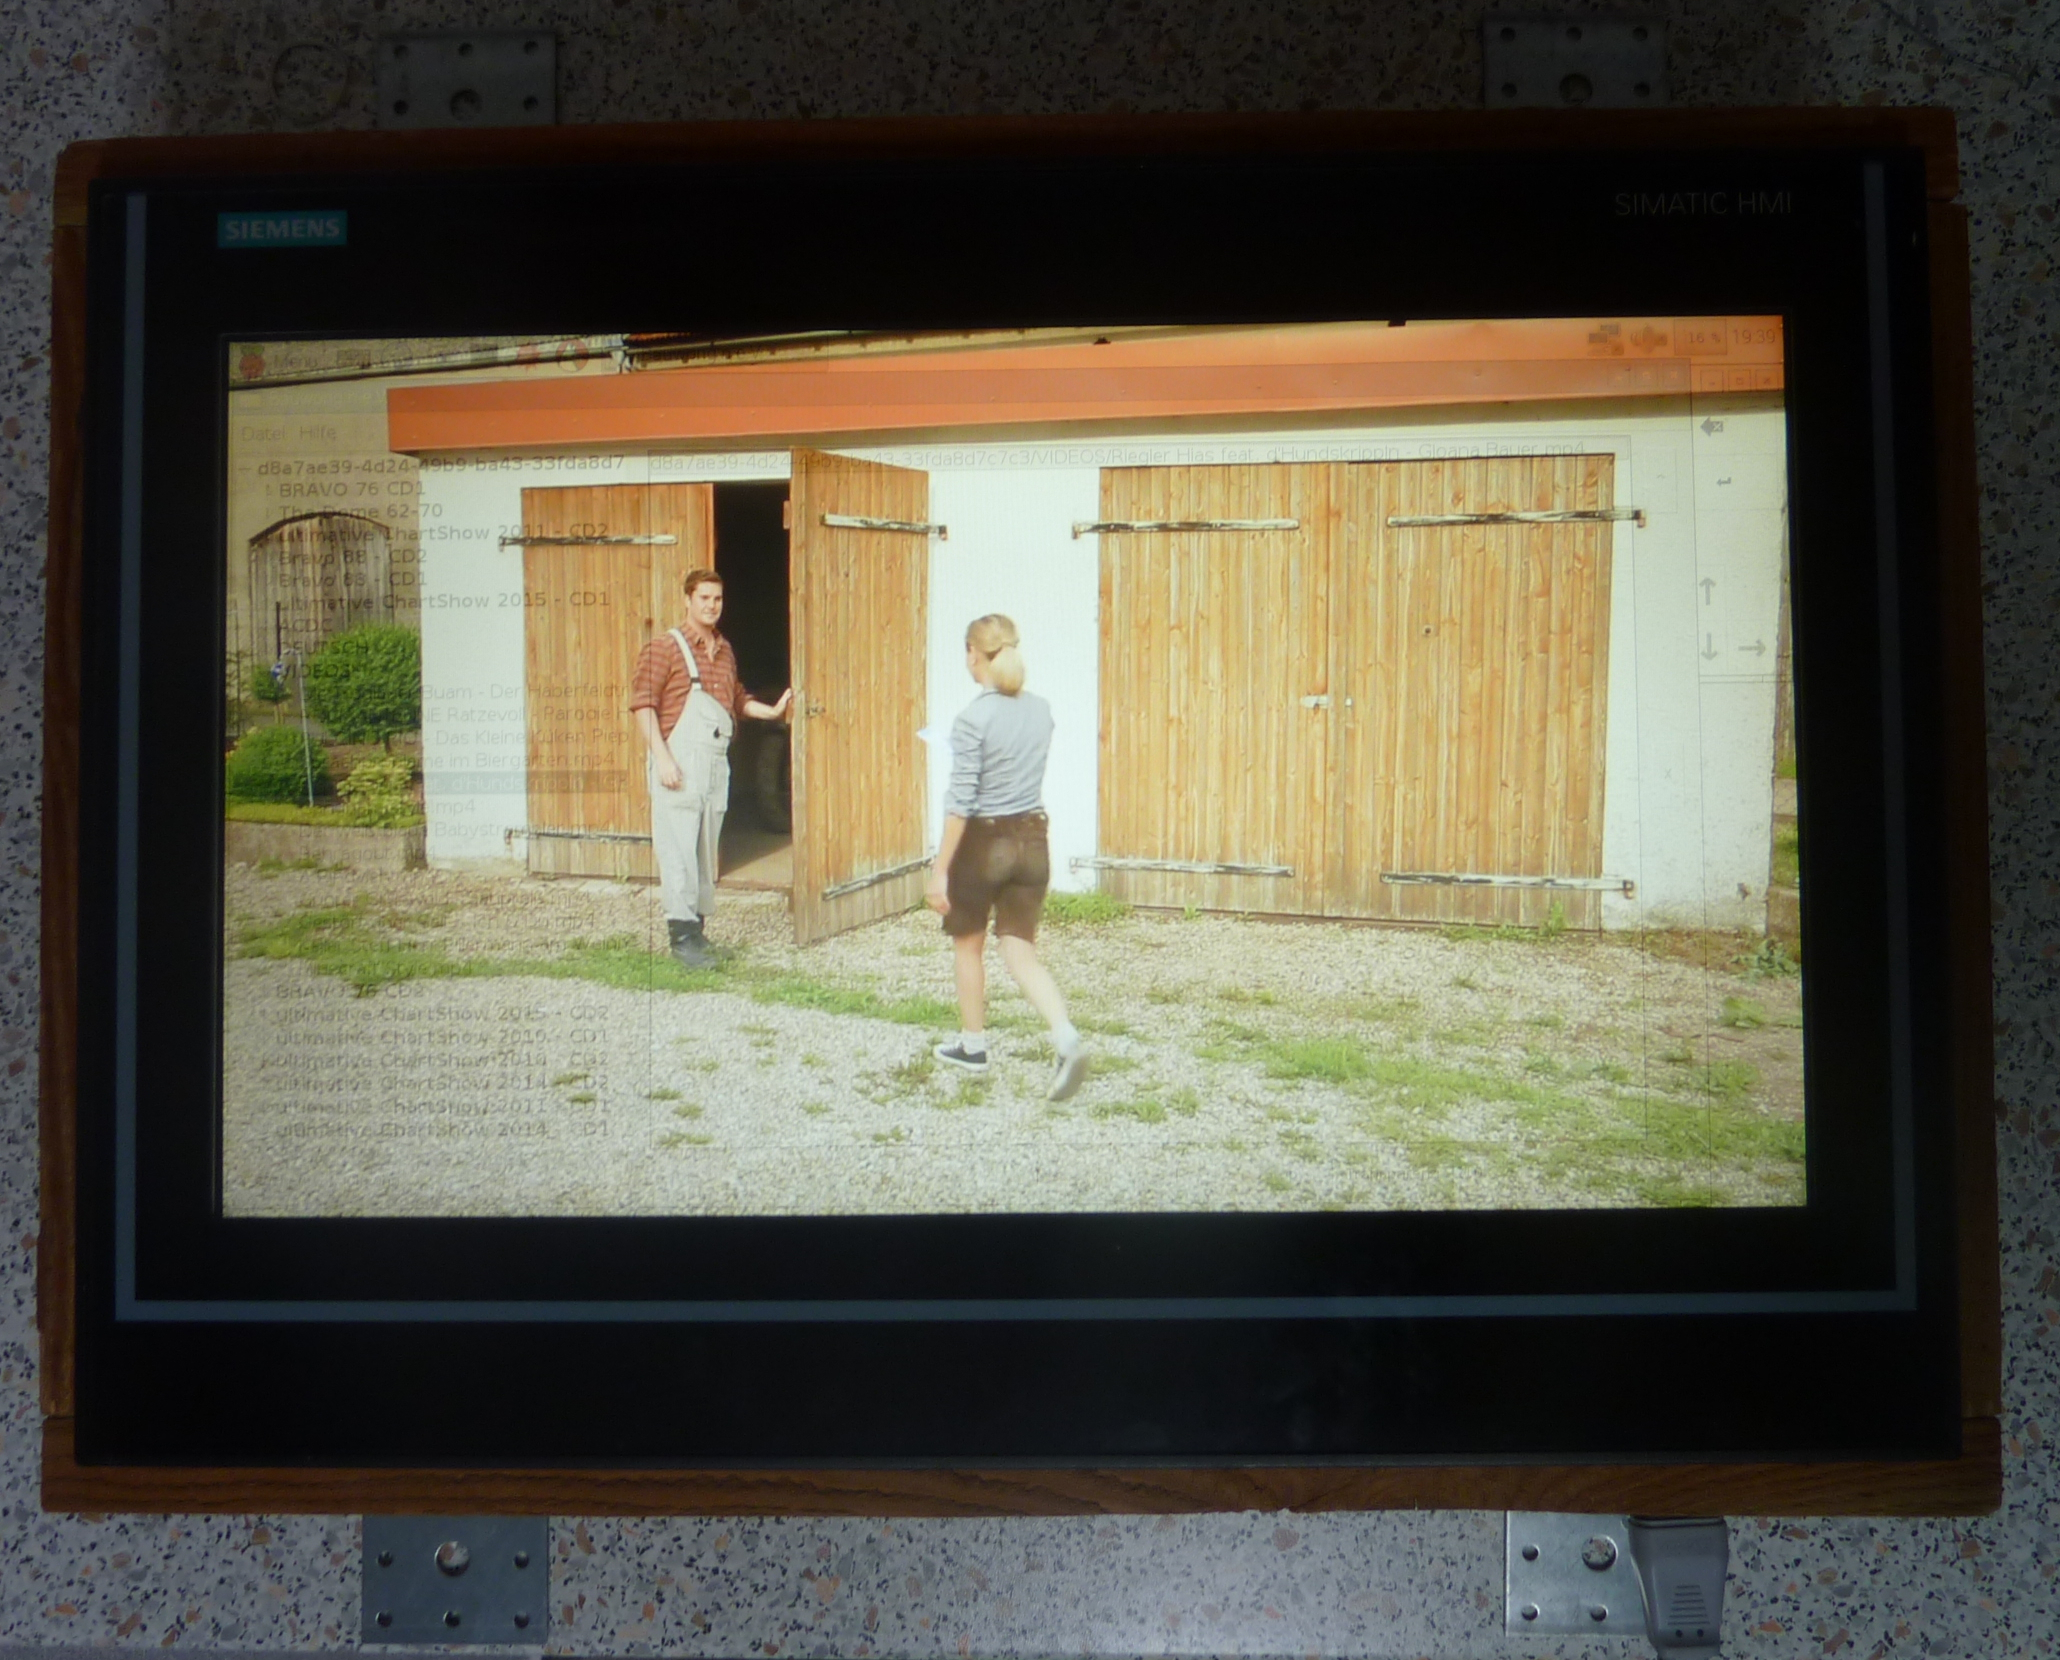
\includegraphics[width=12cm]{Titelbild.jpg}
\end{figure}

%%------------------------------------------------------------------------------
%%   GNU-Logo, Copyrighthinweis, GPLv3-Logo
%%------------------------------------------------------------------------------
\begin{tabular}{lllr}\\
\hline
% --- Zeile mit de offiziellen Logo der Free Software Foundation:
\parbox[c][50px]{0.10\textwidth}{
\includegraphics[height=35px]{GNU.png}} & \parbox[c]{0.40\textwidth}{GNU General Public License v3\\ \copyright\ 2016 - 2017 by \autor}  & \parbox[c]{0.15\textwidth}{Datum:\\18.08.2017} & \parbox[c][50px]{0.20\textwidth}{
\includegraphics[height=35px]{GPLv3.png}}\\
\hline
\end{tabular}

\end{center}

\textbf{}\\
Die Abbildung auf dem Display stammt aus dem Video zu folgendem Musikst�ck:\\
\texttt{\textbf{Riegler Hias feat. d' Hundskrippln} \textit{Gloana Bauer}} bei 2:42\\
\url{https://www.hundskrippln.de/#filme} %-- 2:42

\end{titlepage}




\include{Layout/Abstract}
\cfoot{- \pagemark ~-}

\tableofcontents          % Inhaltsverzeichnis
\listoffigures            % Abbildungsverzeichnis
\listoftables             % Tabellenverzeichnis
\renewcommand{\lstlistlistingname}{Verzeichnis der Listings}
%\lstlistoflistings        % Listings-Verzeichnis

%% Abk�rzungsverzeichnis --------------------------------------------------------
%\input{Kapitel/Glossar}
%% f�r korrekte �berschrift in der Kopfzeile
%\clearpage\markboth{\nomname}{\nomname} 
%\printnomenclature
%\label{sec:Glossar}


% arabische Seitenzahlen im Hauptteil ------------------------------------------
\clearpage
\pagenumbering{arabic}


% ##############################################################################
% ----------   Die Inhaltskapitel werden inkludiert    -------------------------
% ##############################################################################
\chapter{Einf�hrung}
\label{cha:Einfuehrung}

%% Diese Auflistung k�nnte irgendwann notwendig werden,
%% wenn auf Github verschiedene Versionsst�nde herumgeistern und die
%% einzelnen Nutzer evtl. verschiedene St�nde vorliegen haben...
%Ausgabest�nde dieser Dokumentation:
%
%\begin{tabular}{llp{0.70\textwidth}}
%\textbf{Version 1} & 20.02.2016 & Erstversion f�r Programmversion V0.1\\
%\textbf{Version 2} & 01.07.2016 & zus�tzliche Hinweise zur Software-Installation von Version V0.1\\
%\textbf{Version 3} & 18.08.2017 & {\Bezeichnung} {\Version}\\
%\end{tabular}

Diese Dokumentation beschreibt die Installation und Anwendung von {\Bezeichnung}
{\Version} auf einem {\RPi} unter dem Betriebssystem \textit{Raspbian Jessie 
with Desktop (PIXEL)} vom 05.07.2017, Imagedatei 
\textbf{\filenam{2017-07-05-raspbian-jessie.img}}. Um das SD-Image f�r eine 
SD-Karte mit nur 4GB Speicherkapazit�t anzupassen, wurde das Programmpaket 
\textit{Mathematica/Wolfram} (ca. 683MB) gel�scht und das Dateisystem 
entsprechend verkleinert.\\
Die Software wurde auf einem {\RPi} 2B (Quad Core, 900MHz, 1GB RAM) erstellt und
getestet. Auch die Inbetriebnahme auf einem {\RPi} Modell A+ (Single Core, 
700MHz, 512MB RAM) verlief erfolgreich.\\
Nicht gepr�ft wurde hingegen die Lauff�higkeit unter der neuen 
Be\-triebs\-system\-ver\-sion \textit{\mbox{Raspbian} Stretch}, Imagedatei 
\textbf{\filenam{2017-08-16-raspbian-stretch.img}} oder neuer!


\section{Kurzbeschreibung der Software}
\label{sec:Kurzbeschreibung}
"`\Bezeichnung"' \bzw "`\BezeichnungLang"' ist ein in \textbf{Python3}
erstellter Wrapper f�r den Mediaplayer \textbf{\filenam{\omxplayer}}, welcher
optimal auf die Hardware des {\RPi} zugeschnitten ist. Neben der Steuerung des 
nackten \textbf{\filenam{\omxplayer}} �ber Kommandozeilenparameter oder die 
Tastatur ("`hot keys"') ist auch eine Kommunikation mittels \textbf{D-Bus} 
m�glich.\\
Die urspr�ngliche Absicht war, eine Software zu erstellen, mit der eine einfache
und intuitive Handhabung einer Musiksammlung m�glich ist. Dabei sollte sich die
Bedienung an einem klassischen CD-Spieler orientieren. Unter Linux und somit
auch auf dem {\RPi} gibt es das hervorragende Softwarepaket \textbf{MPD} ("`Music
Player Daemon"'), das \ua �ber ALSA alle auf dem Computer installierten
Soundkarten unterst�tzt und zahlreiche Client-Anwendungen (MPC) zur Verf�gung
stellt. Sein einziger Nachteil liegt in der Verwaltung der Musikdateien �ber
eine Datenbank und den damit verbundenen umst�ndlichen und aufw�ndigen
Aktualisierungsarbeiten bei neuen Musikdateien, die dem einfachen
CD-Spieler-Prinzip entgegenstehen. \textit{Gerne lasse ich mich hier vom
Gegenteil �berzeugen, falls es f�r den {\RPi} taugliche MPCs geben sollte, die
obigen Anforderungen gen�gen \smiley{wink}}
(\url{mailto:schlizbaeda@gmx.de}).\\
Die Software \textbf{\Bezeichnung} in Version {\Version} besteht aus einer
grafisch einfach gehaltenen, mit dem Python-Modul \textbf{tkinter} erstellten
Benutzeroberfl�che (GUI) �hnlich einem Dateimanager (siehe Abbildung 
\ref{fig:yamuplay_aufruf}):  Im linken Teil befindet
sich ein sogenanntes Treeview-Steuerelement, in dem die hierarchische
Ordnerstruktur von Laufwerken angezeigt wird, die unter \filenam{/media/pi}
gemountet sind. Am {\RPi} neu angeschlossene USB-Laufwerke werden automatisch
erkannt und entsprechend in die Ordnerstruktur eingebunden. Mediendateien (nicht 
nur Musik, auch Videos) k�nnen durch einen Doppelklick in die Playlist eingef�gt
werden. Links oben ist ein Eingabefeld f�r die Titelsuche enthalten.\\
Der rechte Teil der GUI besteht oben aus den Schaltfl�chen, die den klassischen 
Tasten eines CD-Spielers entsprechen: \textit{Play/Pause}, \textit{fast forward},
\textit{rewind}, Titelsprung und \textit{Stop}. Direkt darunter befindet sich 
eine in {\Version} noch nicht aktive Schiebeleiste, die sp�ter die aktuelle 
Position in der gerade laufenden Mediendatei anzeigen und auch ein schnelles 
Verschieben erm�glichen soll. Rechts unten ist die Playlist, in der alle zum 
Abspielen ausgew�hlten Mediendateien angezeigt werden sowie die Schaltfl�chen zum
Entfernen und Verschieben der Mediendateien. Ein Doppelklick auf eine Mediendatei
der Playlist beendet das laufende St�ck und beginnt mit dem Abspielen des 
angeklickten Titels.\\
Das Men� der GUI erm�glicht unter \menuitem{Datei} das Laden und Speichern von 
Playlists sowie das Beenden der Software. Im Dropdown-Men� \menuitem{Ansicht} 
k�nnen diverse Einstellungen f�r die Wiedergabe von Videodateien eingestellt 
werden. Unter \menuitem{Hilfe} ist derzeit nur die Anzeige einer Aboutbox 
m�glich.\\


\section{Rechtliche Hinweise zu Lizenz, Gew�hrleistung und Links}
\subsection{Software unter GPL v3 }
Die Software \textbf{\Bezeichnung} wird unter der Lizenz GPL v3 der \Verein{Free
Software Foundation} ver�ffentlicht. Sie darf frei kopiert und privat oder 
kommerziell gem�� der Lizenzvorgaben verwendet werden. Bitte lesen Sie die
GPL v3, die sich im Programmpaket in der Datei \filenam{COPYING} befindet
oder laden Sie den Originaltext aus dem Internet von
\url{https://www.gnu.org/licenses/gpl-3.0} herunter.

{\autor} als Urheber und Copyrightinhaber stellt die Software "`so wie sie ist"'
ohne Garantie und ohne Zusicherung einer bestimmten Funktionalit�t zum Download
bereit. Es steht Ihnen als Anwender frei, die Software zu benutzen oder es eben
nicht zu tun. Entscheiden Sie sich f�r die Benutzung, so tun Sie dies auf
eigenes Risiko und auf eigene Verantwortung. Der Autor �bernimmt keine Garantie
f�r die Software und deren Funktion und haftet auch nicht f�r Sch�den, die aus
der Installation und Verwendung der Software entstehen.

\subsection{Dokumentation unter FDL v1.3}
Diese Dokumentation wurde mit dem Textsatzsystem {\LaTeX} erstellt.\\
Sie darf gem�� der Bestimmungen aus der Lizenz FDL v1.3 (oder nachfolgend)
kopiert, verteilt und/oder ge�ndert werden. Details siehe 
\url{http://www.gnu.org/licenses/fdl.html}

\subsection{Externe Internet-Links}
\textbf{Einfach weil's sein muss:}\\
In diesem Dokument befinden sich Hyperlinks zu verschiedenen externen Seiten 
anderer Anbieter im Internet, die au�erhalb des Verantwortungsbereiches des 
Autors liegen. Durch die blo�e Anbringung eines Links auf eine fremde Seite 
macht sich der Autor deren Inhalte nicht zu eigen, da er auf die Gestaltung 
dieser Seiten keinerlei Einfluss hat. Zum Zeitpunkt der Verlinkung waren auf 
den verlinkten Seiten keine illegalen Inhalte erkennbar. Sollten aktuelle
oder k�nftige Inhalte jedoch rechtswidrig sein, so kann der Autor dar�ber
per e-mail an \url{mailto:schlizbaeda@gmx.de} informiert werden. Es werden
dann entsprechende Ma�nahmen zur Beseitigung des/der betroffenen Links ergriffen.


\section{Konventionen dieser Dokumentation}
Folgende gestalterische Konventionen werden f�r die Dokumentation festgelegt:

\begin{table}[!h]
\centering
\renewcommand{\arraystretch}{2}
\begin{tabular}{|p{3.5cm}|p{10.5cm}|}
\hline
\parbox[c]{1em}{\begin{bclogo}[logo = \bclampe, noborder = true]{Hinweis}
Text
\end{bclogo}}
	& Ein Hinweis enth�lt zus�tzliche Information bzw. relevante Erl�uterung zu einer bestimmten Funktionalit�t\\
\hline
\parbox[c]{3.5cm}{\begin{bclogo}[arrondi = 0.2, logo = \bcinfo, ombre = true, epOmbre = 0.25, couleurOmbre = black!30,blur]{Achtung}
Text
\end{bclogo}}	& Ein Warnhinweis, dessen Nichtbeachtung zu Ger�tesch�den f�hren kann\\
\hline
\button{Schaltfl�che} & Kennzeichnung von Schaltfl�chen der Software \textbf{\Bezeichnung}\\
\hline
\menuitem{Men�punkt} & {Kennzeichnung von Men�punkten der Software \textbf{\Bezeichnung}}\\
\hline
\prompt{Meldung} & Kennzeichnung von Meldungen der Software \textbf{\Bezeichnung}\\
\hline
\end{tabular}
\vspace{0.5cm}
\caption{Konventionen der Dokumentation}
\end{table}


\newpage
\section{Abk�rzungsverzeichnis}
Folgende Abk�rzungen werden in dieser Dokumentation verwendet:
\begin{acronym}[\Bezeichnung]
	\acro{ALSA}{\textbf{A}dvanced \textbf{L}inux \textbf{S}ound \textbf{A}rchitecture}
	\acro{D-Bus}{\textbf{D}esktop-\textbf{Bus}}
%	\acro{DVI}{\textbf{D}igital \textbf{V}isual \textbf{I}nterface}
	\acro{GUI}{\textbf{G}raphical \textbf{U}ser \textbf{I}nterface}
	\acro{HDMI}{\textbf{H}igh \textbf{D}efinition \textbf{M}ultimedia \textbf{I}nterface}
	%\acro{mP}{\textbf{M}ikro \textbf{P}rozessor}
	\acro{MPC}{\textbf{M}usic \textbf{P}layer \textbf{C}lient}
	\acro{MPD}{\textbf{M}usic \textbf{P}layer \textbf{D}aemon}
	\acro{SoC}{\textbf{S}ystem \textbf{o}n \textbf{S}ilicon: {\textmu}P-Bausteine mit viel Peripheriemodulen wie \zB der Broadcom 2835, 2836, 2837 auf dem \RPi}
%	\acro{USV}{\textbf{U}nterbrechnungsfreie \textbf{S}trom\textbf{v}ersorgung}
\end{acronym}


\section{Danksagung}
Mein Dank gilt insbesondere folgenden Personen
\begin{itemize}
\item \textbf{\textit{Riegler Hias} und \textit{d' Hundskrippln}}\\
     In dieser Dokumentation wird an verschiedenen Stellen auf das Musikst�ck
     \textit{Gloana Bauer} von \textbf{Riegler Hias feat. d' Hundskrippln} 
     verwiesen, weil ich dieses Lied einfach gut finde.\\
     \begin{tabular}{ll}
     \url{https://www.hundskrippln.de} & 93336 Steinsdorf\\
     \url{http://www.riegler-hias.de}  & 93349 Hiendorf\\
     \end{tabular}
     
     Ich bedanke mich f�r die Erlaubnis, Screenshots aus dem Video zu diesem
     Musikst�ck verwenden zu d�rfen.
\item \textbf{meigrafd}\\
     Dieser Benutzer des gr��ten deutschsprachigen Forums f�r den {\RPi} lud 
     damals offenbar die Version V0.1 von {\Bezeichnung} herunter und testete 
     es anschlie�end ziemlich ausf�hrlich durch. Er lie� mir �u�erst 
     konstruktive Kritik zukommen, an welchen Stellen mein urspr�ngliches 
     Python-Script noch zu verbessern w�re.\\
     Insbesondere  schlug er mir vor, meinen damaligen Code von klassischem 
     Python mit unz�hligen \Code{global}-Deklarationen auf objektorientierte 
     Programmierung umzustellen. Dazu hatte er \textit{einfach so} mein 
     komplettes Script angepasst und mir wieder zukommen lassen. Darauf 
     aufbauend korrigierte und erweiterte ich das Script auf den jetzigen
     Versionsstand {\Version}.
     \url{http://www.forum-raspberrypi.de/User-meigrafd}
\end{itemize}

\chapter{Software \Bezeichnung}
\label{cha:Software}

%%%%%%%%%%%%%%%%%%%%%%%%%%%%%%%%%%%%%%%%%%%%%%%%%%%%%%%%%%%%%%%%%%%%%%%%%%%%%%%%
\section{Installation von \Bezeichnung}
{\Bezeichnung} wird von {\autor} unter {\github} unter 
\url{https://github.com/schlizbaeda/yamuplay} zum Download bereitgestellt. 
Das Softwarepaket besteht im Wesentlichen aus dem Python3-Script 
\filenam{yamuplay.py} und einigen Zusatzdateien sowie dem {\LaTeX}-Quellcode
dieser Dokumentation.\\
Damit das Python3-Script auf dem {\RPi} lauff�hig wird, m�ssen weitere 
Python-Mo\-du\-le installiert werden, die ebenfalls auf {\github} verf�gbar sind
oder als Paket in Raspbian enthalten sind:

\begin{table}[h]
\centering
\renewcommand{\arraystretch}{1.25}
\begin{tabular}{lll}
\textbf{Python-Modul} & \textbf{Lizenz} & \textbf{Quelle}\\
python-omxplayer-wrapper & LGPL v3 & \scriptsize{\url{https://github.com/willprice/python-omxplayer-wrapper.git}}\\
python3-dbus & MIT & \filenam{apt-get install python3-dbus}\\
pyudev v0.21.0 & LGPL v2.1 & \url{https://github.com/pyudev/pyudev.git}\\
python-magic & MIT & \url{https://github.com/ahupp/python-magic.git}\\
\end{tabular}
\vspace{0.25cm}
\caption{Zus�tzliche Python-Module f�r den Betrieb von {\Bezeichnung}}
\end{table}
%------------------------------------------------------------------------------%
\subsection*{Installation}
Auf einem {\RPi}, der mit dem Internet verbunden ist, kann die Installation in
einem Terminalfenster durch Eingabe folgender Anweisungen durchgef�hrt werden:

Programmpaket \textbf{\Bezeichnung}\\
\verb|  cd /home/pi|\\
\verb|  git clone https://github.com/schlizbaeda/yamuplay.git|\\
\verb|  cd yamuplay|\\
\verb|  chmod 755 yamuplay.py|

Programmpaket \textbf{python-omxplayer-wrapper}\\
\verb|  cd /home/pi/yamuplay|\\
\verb|  git clone https://github.com/willprice/python-omxplayer-wrapper.git|\\
\verb|  cd python-omxplayer-wrapper|\\
\verb|  sudo python3 setup.py install|

Programmpaket \textbf{python3-dbus}\\
\verb|  cd /home/pi/yamuplay|\\
\verb|  sudo apt-get install python3-dbus|

Programmpaket \textbf{pyudev v0.21.0}\\
\verb|  cd /home/pi/yamuplay|\\
\verb|  git clone https://github.com/pyudev/pyudev.git|\\
\verb|  cd pyudev|\\
\verb|  sudo python3 setup.py install|

Programmpaket \textbf{python-magic}\\
\verb|  cd /home/pi/yamuplay|\\
\verb|  git clone https://github.com/ahupp/python-magic.git|\\
\verb|  cd python-magic|\\
\verb|  sudo python3 setup.py install|

\subsection*{Programmaufruf}
Der Start von {\Bezeichnung} erfolgt �ber das Kommando\\
\verb|  /home/pi/yamuplay/yamuplay.py|
\begin{figure}[h]
\centering
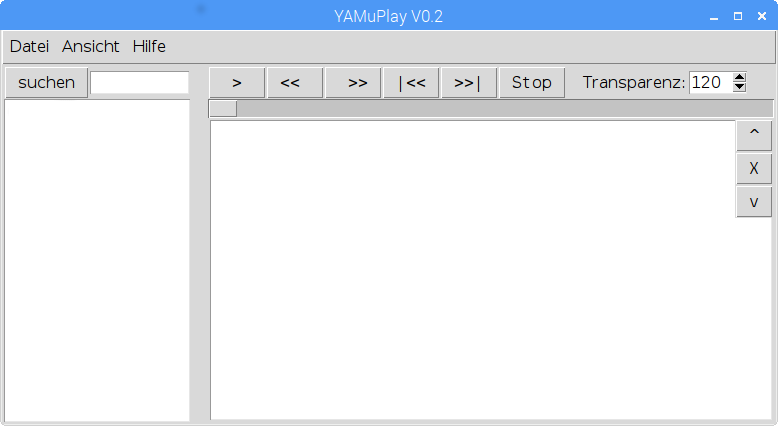
\includegraphics[width=\textwidth]{yamuplay_aufruf.png}
\caption{Erstmaliger Aufruf von \Bezeichnung}
\label{fig:yamuplay_aufruf}
\end{figure}


%%%%%%%%%%%%%%%%%%%%%%%%%%%%%%%%%%%%%%%%%%%%%%%%%%%%%%%%%%%%%%%%%%%%%%%%%%%%%%%%
\section{Beschreibung und Bedienung von \Bezeichnung}
Die Software {\Bezeichnung} {\Version} ist kein eigener Mediaplayer, sondern 
eine Bedieneroberfl�che f�r den existierenden Kommandozeilen-Mediaplayer
{\filenam{\omxplayer}, der in den meisten(?) Betriebssystem-Distributionen
f�r den {\RPi} standardm��ig enthalten ist. Diese Oberfl�che ist quasi eine
"`H�lle"' -- oder auf englisch -- ein \textit{Wrapper} f�r {\filenam{\omxplayer}.
Der Sinn f�r die Programmierung von {\Bezeichnung} lag \ua darin, eine Plattform
unter \textbf{Python3} zu schaffen, mit der man relativ einfach Mediendateien
(Musik und Videos) unter Zuhilfenahme von {\filenam{\omxplayer} abspielen
kann. Da \filenam{\omxplayer} als eigener Prozess gestartet wird und die
Kommunikation mit {\Bezeichnung} �ber \textbf{D-Bus} erfolgt, findet das
Abspielen aus der Sicht des �bergest�lpten Python-Scripts im Hintergrund
statt; in Python k�nnen w�hrenddessen andere Aufgaben erledigt werden. Ein
weiterer Vorteil liegt darin, dass \filenam{\omxplayer} haupts�chlich den
GPU-Teil des SoC \textit{Broadcom 283x} auf dem {\RPi} beansprucht und somit 
den CPU-Teil kaum belastet. Die CPU-Last beim Betrieb von {\Bezeichnung} liegt 
auf ei\-nem {\RPi} 1 mit dem Broadcom-SoC 2835 bei ca. 25\%-35\%, es bleiben 
gen�gend CPU-Res\-sour\-cen frei.\\
Nachteilig ist jedoch, dass ALSA aufgrund der gro�en Hardwaren�he von
\filenam{\omxplayer} nicht eingebunden ist und somit wirkungslos bleibt.
Daher funktioniert weder der ALSA-Mixer von Raspbian, noch kann eine Soundkarte
wie Hifiberry DAC+ eingesetzt werden. Die Audioausgabe kann nur �ber HDMI
oder den Analoganschluss des {\RPi} erfolgen, eine Laust�rkeregelung muss am
Audioverst�rker vorgenommen werden!

%------------------------------------------------------------------------------%
\subsection{Bedienkonzept}
Es gibt bereits gen�gend kompliziert zu bedienende Mediaplayer vor allem
hinsichtlich der Erstellung, �nderung und Verwaltung von Playlists. Bereits
in Kapitel \ref{sec:Kurzbeschreibung} wurde die Problematik des
Music Player Daemons angedeutet, insbesondere wenn �nderungen in der Liste der
abzuspielenden St�cke \textit{schnell} vorgenommen werden sollen/m�ssen. 
Vielmehr ist in solchen F�llen eine intuitive Bedieneroberfl�che erforderlich.
{\Bezeichnung} ist ein Versuch in diese Richtung, aber auch hier k�nnte noch 
viel getan werden, das will ich gar nicht abstreiten. Weitere geplante 
Verbesserungen dazu f�r k�nftige Programmversionen sind in Kapitel 
\ref{sect:Erweiterungen} aufgef�hrt.


%------------------------------------------------------------------------------%
\subsection{Aufbau der GUI}
Das Hauptfenster von {\Bezeichnung} ist zweigeteilt, siehe Abbildung
\ref{fig:yamuplay_controls}. Die wichtigsten Steuerelemente zur Bedienung von 
{\Bezeichnung} befinden sich auf der grafischen Oberfl�che und k�nnen direkt 
durch Anklicken bedient werden.
\begin{figure}[h]
\centering
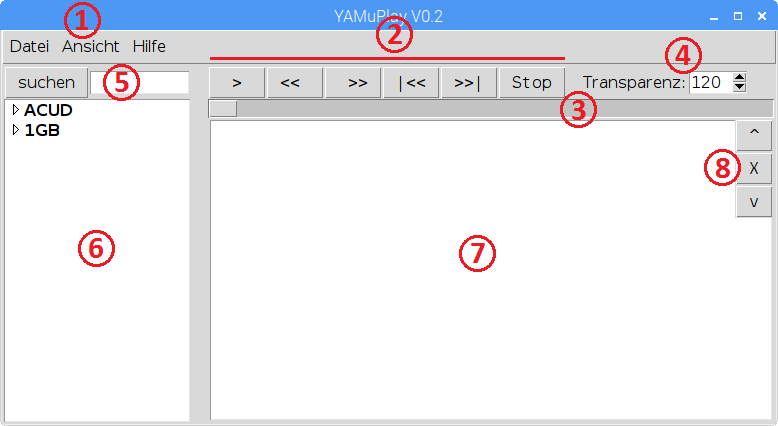
\includegraphics[width=\textwidth]{yamuplay_controls.png}
\caption{Steuerelemente in der Benutzeroberfl�che von \Bezeichnung}
\label{fig:yamuplay_controls}
\end{figure}

\begin{table}[h]
\centering
\renewcommand{\arraystretch}{1.25}
\begin{tabular}{ll}
\textbf{(1)} & Hauptmen�\\
\textbf{(2)} & an einen CD-Spieler angelehnte Schaltfl�chen\\
\textbf{(3)} & Fortschrittsbalken f�r die laufende Mediendatei -- \textbf{derzeit noch inaktiv}\\
\textbf{(4)} & Einstellung f�r den Alphawert (Transparenz) von angezeigten Videos\\
\textbf{(5)} & Titelsuche\\
\textbf{(6)} & Anzeige der Dateien auf den angesteckten USB-Laufwerken\\
\textbf{(7)} & Playlist\\
\textbf{(8)} & Steuerelemente zum L�schen oder Verschieben von Elementen der Playlist\\
\end{tabular}
\vspace{0.25cm}
\caption{Steuerelemente in der Benutzeroberfl�che von \Bezeichnung}
\end{table}
In der linken H�lfte werden alle auf den
angeschlossenen USB-Laufwerken enthaltenen Dateien und Verzeichnisse in einer
hierarchischen Baumstruktur angezeigt, gew�hnliche Dateien in Normalschrift und
Verzeichnisse in fetter Schrift. Ein Doppelklick auf ein Verzeichnis �ffnet oder
schlie�t es, eine gew�hnliche Datei wird der Playlist hinzugef�gt. Mehrmaliges
Hinzuf�gen der gleichen Datei zur Playlist ist nat�rlich m�glich. {\Bezeichnung}
kann derzeit jedoch noch nicht unterscheiden, ob es sich bei der gew�hlten Datei
um eine abspielbare Mediendatei oder um einen anderen Dateityp (\zB eine
Textdatei) handelt.\\ 
Im oberen Bereich befinden sich Steuerelemente zur Dateisuche. Die Suche
ber�cksichtigt derzeit nur die \textbf{Dateinamen}, nicht die Metadaten
(\zB ID3-Tags) der Mediendateien. Dies w�rde ja eine Datenbank erfordern, auf
die aus Performancegr�nden bewusst verzichtet wurde. \\
Wird ein USB-Laufwerk entfernt oder ein weiteres angeschlossen, so wird die
Baumstruktur entsprechend aktualisiert. Dateieintr�ge in der Playlist bleiben
davon unangetastet!

Der rechte Teil enth�lt oben die Schaltfl�chen \textit{Play/Pause}, 
\textit{seek}, \textit{prev}, \textit{next} und \textit{Stop}, die den Tasten 
eines CD-Spielers nachempfunden sind und (hoffentlich) keiner Erkl�rung 
bed�rfen \smiley{smile} 
Direkt darunter ist ein derzeit noch inaktiver Fortschrittsbalken, der in 
folgenden Programmversionen die aktuelle Position des laufenden St�cks anzeigen
und auch ein Verschieben erm�glichen soll.\\
Neben den CD-Schaltfl�chen befindet sich ein Eingabefeld f�r die Transparenz 
(den sogenannten alpha-Wert) von Videos, die zwischen 0 (vollst�ndig transparent,
\dahe unsichtbar) und 255 (vollst�ndig deckend) liegen kann. Grunds�tzlich 
reagiert der Desktop auch bei deckender Anzeige von Videos auf Maus- \bzw 
Touchereignisse ganz normal, die Eingabe muss allerdings "`blind"' erfolgen. 
Der Standardwert von 120 f�r die Transparenz l�sst den Desktop des {\RPi} und 
{\Bezeichnung} noch leicht durchscheinen, so dass eine optische Bedienung 
m�glich ist.
Der untere Teil wird vollst�ndig von der Playlist ausgef�llt, in der die 
aktivierten Mediendateien angezeigt werden. Am rechten Rand befinden sich 
Schaltfl�chen, um einzelne Dateien in der Liste zu verschieben oder wieder 
ganz aus der Liste zu entfernen. Ein Doppelklick auf einen Titel in der Playlist 
springt sofort dorthin und spielt diesen Titel ab.\\


%------------------------------------------------------------------------------%
\subsection{Men�}
DropDown-Men� \textbf{Datei}
\begin{itemize}
\item{\textbf{Datei$\rightarrow$Playlist �ffnen}\\
      Laden einer gespeicherten Playlist:\\
      Es wird der Standarddialog des Betriebssystems zur Dateiauswahl angezeigt,
      mit dem der Dateiname ausgew�hlt werden kann. Das Dateiformat ist 
      \Code{m3u}, eine Textdatei, in der jede Zeile eine Mediendatei enth�lt.
      \begin{bclogo}[logo = \bclampe, noborder = true]{Hinweis}
      Die bestehende Playlist in {\Bezeichnung} wird dabei nicht gel�scht, sondern
      die in der Play\-list-Da\-tei enthaltenen Mediendateien werden hinten 
      angeh�ngt.
      \end{bclogo}}
\item{\textbf{Datei$\rightarrow$Playlist speichern}\\
      Speichern der aktuellen Playlist:\\
      Es wird der Standarddialog des Betriebssystems zur Dateiauswahl angezeigt,
      mit dem der Dateiname der \Code{m3u}-Da\-tei ausgew�hlt werden kann. Es
      werden alle Elemente der aktuellen Playlist von {\Bezeichnung} 
      abgespeichert.}
\item{\textbf{Datei$\rightarrow$Beenden}\\
      {\Bezeichnung} verlassen}
\end{itemize}

\newpage
DropDown-Men� \textbf{Ansicht}
\begin{bclogo}[logo = \bclampe, noborder = true]{Hinweis}
Dieses Men� beinhaltet Punkte zur Steuereung der Videodarstellung. F�r reine
Musikdateien wird es nicht ben�tigt.
\end{bclogo}
\begin{itemize}
\item{\textbf{Ansicht$\rightarrow$Vollbild}\\
      Wechsel zwischen der Anzeige eines Videos als Vollbild oder in einem 
      Fenster}
\item{\textbf{Ansicht$\rightarrow$AspectMode}\\
      Einstellung der Darstellungsanpassung von Videos mit den drei Modes
      \textit{letterbox}, \textit{fill} und \textit{stretch}:\\
      \textit{letterbox:}\\
      Vollst�ndige Skalierung in das Videofenster ohne Verzerrung. Es entstehen
      R�nder an der zu gro�en Seite.\\
      \textit{fill:}\\
      Skalierung in das Videofenster auf die kleinere Kante. Zu gro�e Bereiche 
      werden abgeschnitten und sind unsichtbar.\\
      \textit{stretch:}\\
      Anpassung an die Fenstergr��e mit Verzerrung}
\item{\textbf{Ansicht$\rightarrow$Hintergrundfarbe}\\
      �ber den Standarddialog "`Farbauswahl"' des Betriebssystems kann eine
      Hintergrundfarbe f�r das Videofenster gew�hlt werden. Bei alpha-Wer\-ten
      kleiner als 255 schimmert die Hintergrundfarbe anteilig durch das Video.
      Damit k�nnen nette(?) Effekte erzeugt werden \smiley{lol}}
\item{\textbf{Ansicht$\rightarrow$Videogr��e automatisch anpassen}\\
      Normalerweise wird die Fenstergr��e bei Neustart einer Videodatei auf die
      Originalgr��e des Videos angepasst und mittig dargestellt. Da dies aber 
      auch unerw�nscht sein kann, werden alle Videos an die vom Anwender 
      eingestellte Gr��e unter Ber�cksichtigung des "`Aspect Mode"' angepasst.}
\end{itemize}

DropDown-Men� \textbf{Hilfe}
\begin{itemize}
\item{\textbf{Hilfe$\rightarrow$Info}\\
      Anzeige einer sogenannten "`Aboutbox"', in der Informationen �ber die 
      Software und die Lizenz von {\Bezeichnung} angezeigt werden (siehe 
      Abbildung \ref{fig:yamuplay_info})}
\end{itemize}
\begin{figure}[h]
\centering
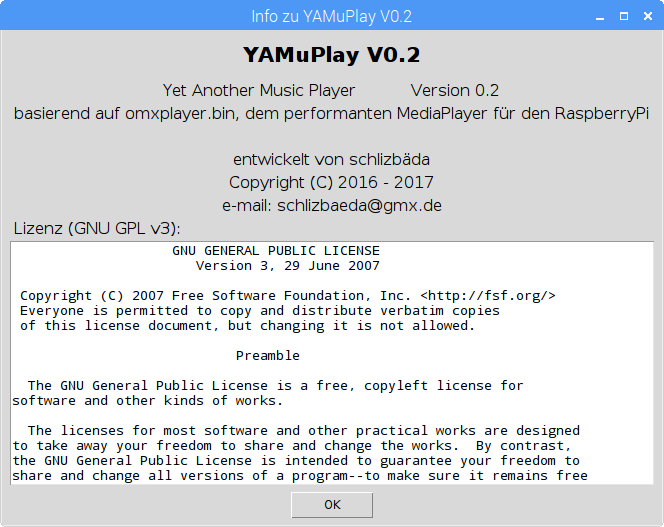
\includegraphics[width=\textwidth]{yamuplay_info.png}
\caption{Aboutbox von \Bezeichnung}
\label{fig:yamuplay_info}
\end{figure}


\newpage
%------------------------------------------------------------------------------%
\subsection{Bedienung �ber die Tastatur}
Die Bedienung von {\Bezeichnung} ist weitestgehend auch �ber die Tastatur 
m�glich. Die Taste \button{TAB} erm�glicht (wie bei den meisten Programmen mit 
einer GUI) das Wechseln des aktiven Steuerelementes. In der Playlist und im 
Tree\-view-Steu\-er\-e\-le\-ment und kann mit den Cursortasten eine Datei gew�hlt 
werden. Ein Directory kann dabei mit \button{Cursor links} und \button{Cursor 
rechts} auf- oder zugeklappt werden.

Ferner sind einige Funktionstaten wir folgt belegt:\\
\begin{table}[h]
\centering
\renewcommand{\arraystretch}{1.25}
\begin{tabular}{ll}
\button{F1}  & Anzeige der Aboutbox (Men�punkt Hilfe-->Info)\\
\button{F2}  & Debugausgabe im Konsolenfenster: def omxplayerDebugPrint(self):\\
\button{F9}  & Transparenz auf Defaultwert setzen (Kommandozeilenparameter -alpha)\\
\button{F10} & �ffnen des Men�s (offenbar ein internes TKinter-Feature)\\
\button{F11} & Wechsel zwischen Videoanzeige im Fenster und Vollbild\\
\button{F12} & Wechsel der "aspect modes": letterbox, fill, stretch\\
\end{tabular}
\vspace{0.25cm}
\caption{Funktionstastenbelegung in \Bezeichnung}
\end{table}

\begin{bclogo}[logo = \bclampe, noborder = true]{Hinweis}
Ein hoher alpha-Wert (wenig Transparenz) kann vor allem bei Vollbildanzeige oder
gro�en Videofenstern die Bedienung einschr�nken. Durch Dr�cken von \button{F9}
wird der alpha-Wert auf einen einstellbaren Standardwert (normalerweise 120) 
gesetzt. Damit ist eine Bedienung der Oberfl�che wieder einigerma�en m�glich,
da die transparente Videodarstellung den Desktop durchscheinen l�sst.
\end{bclogo}

\begin{figure}[h]
\centering
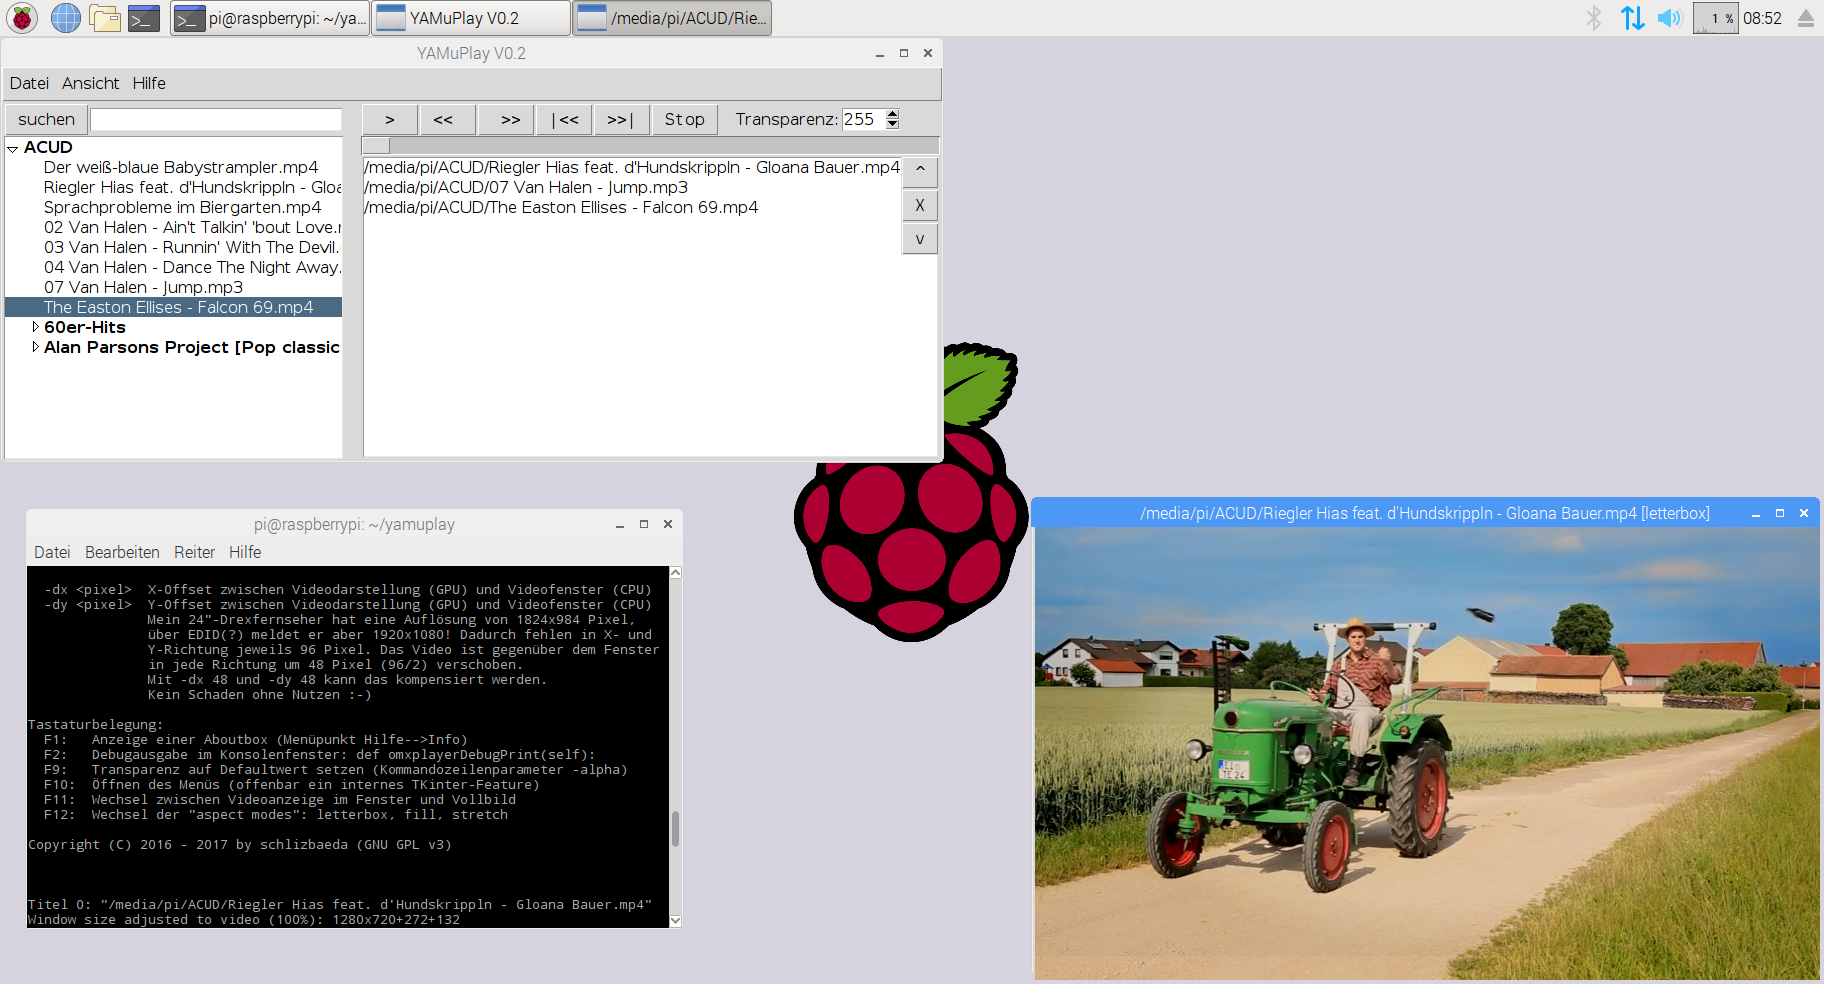
\includegraphics[width=\textwidth]{yamuplay_videobox.png}
\caption{Video mit {\Bezeichnung} in einem Fenster abspielen}
\label{fig:yamuplay_videobox}
\end{figure}


%------------------------------------------------------------------------------%
\subsection{Aufruf im Terminalfenster und Kommandozeilenparameter}
Der Start von {\Bezeichnung} erfolgt im Terminal �ber die Kommandos\\
\verb|  cd /home/pi/yamuplay|\\
\verb|  ./yamuplay.py [Parameter] [Mediadatei(en)]|

Nach dem Programmstart wird im Terminalfenster eine kurze Hilfe ausgegeben,
in der \ua die Aufrufparameter beschrieben werden.
\newpage
\begin{table}[h]
\centering
\renewcommand{\arraystretch}{1.25}
\begin{tabular}{ll}
\verb|-f <bool>    | & 0=Videoanzeige im Fenster, 1=Videoanzeige als Vollbild\\
\verb|-a <mode>    | & \textit{aspect mode} mit den Optionen \textit{letterbox}, \textit{fill} und \textit{stretch}\\
\verb|-k <bool>    | & 0=Videofenster an die Gr��e des Videos anpassen,\\
\verb|             | & 1=Gr��e des Videofensters nicht anpassen\\
\verb|-c <backcol> | & Hintergrundfarbe des Videofensters festlegen\\
\verb|-alpha <int> | & alpha-Standardwert f�r Druck von \button{F9} festlegen\\
\verb|-dx <pixel>  | & X-Versatz zwischen GPU und CPU\\
\verb|-dy <pixel>  | & Y-Versatz zwischen GPU und CPU
\end{tabular}
\vspace{0.25cm}
\caption{Kommandozeilenparameter von \Bezeichnung}
\end{table}

\begin{bclogo}[logo = \bclampe, noborder = true]{Hinweis}
Bei Betrieb des {\RPi} an einem FullHD-Fernsehger�t mit einer nominalen Aufl�sung
von 1920x1080 anstelle eines Computermonitors ist ein Versatz von \Code{-dx 48}
und \Code{-dy 48} zu verwenden, um die Videoausgabe durch die GPU mit dem von der
CPU angezeigten Videofenster in Deckung zu bringen.
Die \textit{echte} Aufl�sung eines FullHD-Fernsehers betr�gt offenbar nur
1824x984 Pixel.
\end{bclogo}

Im weiteren Betrieb von {\Bezeichnung} dient das Terminalfenster auch zur Ausgabe
von Debuginformationen. Mit der Taste \button{F2} erfolgt die in der Routine
\Code{def omxplayerDebugPrint(self):} programmierte Debugausgabe im Terminal.
Au�erdem machen viele Routinen Debugausgaben der von ihnen ermittelten Werte. 


%%%%%%%%%%%%%%%%%%%%%%%%%%%%%%%%%%%%%%%%%%%%%%%%%%%%%%%%%%%%%%%%%%%%%%%%%%%%%%%%
\section{Erweiterungen und Verbesserungen der Software}
\label{sect:Erweiterungen}
Zuletzt noch eine Liste von Punkten, um die das Python3-Script \filenam{yamuplay.py} 
erg�nzt werden k�nnte. Hier handelt es sich um ein \textit{Brainstorming}. Die
Reihenfolge soll keine Gewichtung darstellen!

\begin{itemize}
\item \textbf{FEHLER:\\Das Schlie�en des Videofensters mit dem roten "`X"' f�hrt zu einer Script-Fehlermeldung!}\\
      Ein Umschalten von Vollbild in Fensteransicht ist nicht mehr m�glich, da das Fenster geschlossen wurde.\\
      --> nicht schlie�en, sondern minimieren?
\item \textbf{Tastaturbedienung erweitern}\\
      Durch Dr�cken von \button{ENTER} oder \button{Space} soll der aktuelle
      Listeneintrag (Treeview, Playlist) aktiviert werden. Identisch zu
      Doppelklick
\item \textbf{Scrolling durch Wischgesten wie an einem Smartphone}\\
      horizontal und vertikal: \Code{Treeview.xview} bzw. \Code{Treeview.yview}
\item \textbf{Scrollbalken f�r Treeview und Playlist}\\
      horizontal und vertikal, da die Schrift der Listeneintr�ge wegen der 
      vorgesehenen Touchbedienung relativ gro� ist.
\item \textbf{Auf die Gesamtdauer eines St�ckes skalierter "`Fortschrittsbalken"'}\\
      einfache Verschiebem�glichkeit mit Zeitanzeige wie bei den meisten Mediaplayern
      Das Steuerelement existiert bereits, hat aber noch keine Funktion!
\item \textbf{Anzeige von Titelnummer und aktueller Laufzeit}\\
      wie bei den meisten klassischen CD-Spielern
\item \textbf{\textit{Drag + Drop} von Mediendateien aus der Baumstruktur in die Playlist}\\
      Damit h�tte man die M�glichkeit, neue Titel irgendwo in der Mitte der
      bestehenden Playlist einzuf�gen. Momentan werden alle neuen Titel hinten
      angeh�ngt.
\item \textbf{Lautst�rke �ber \filenam{\omxplayer} einstellen}\\
      \textbf{WICHTIG:}\\
      ALSA funktioniert wegen der Hardwaren�he von \filenam{\omxplayer} nicht!
\item \textbf{omxplayer-eigenes Fading beseitigen (falls m�glich)}\\
      Der \filenam{\omxplayer} macht ein kurzes Fading (< 1 Sekunde) beim Start
      einer neuen Musikdatei. Dies ist manchmal wirklich st�rend!\\
      Komischerweise nicht bei Videodateien
\item \textbf{PLAYLIST}\\
      * bereinigen um nicht mehr vorhandene oder ung�ltige Dateien\\
      * Dateien �ber Men� auch aus Orten ungleich \filenam{/media/pi/...} laden\\
      * bei zweitem Aufruf von {\Bezeichnung} die Dateien aus den Kommandozeilenparametern an die Playlist anh�ngen.\\
      * Bei angegebenen Kommandozeilenparametern sofort nach dem Programmstart mit dem Abspielen beginnen\\
      * BILDER als Diashow anzeigen (Zeit �ber Men�/cmdlin einstellbar)
\item \textbf{Schriftgr��e anpassen auf unterschiedliche Displaygr��en}\\
      \textbf{schwierig:}\\
      Schriftgr��e vor allem f�rs Treeview-Steuerelement parametrierbar machen 
\item \textbf{Erkennung anderer USB-Ger�tetypen (Smartphones)}\\
      Derzeit wird nur der USB-Ger�tetyp "`Mass Storage Device"' unterst�tzt.
      Viele neuere Smartphones stellen ihre Daten mitunter nur noch �ber MTP
      (Media Transfer Protocol), eine Weiterentwicklung von PTP (Picture
      Transfer Protocol) zur Verf�gung.
\item \textbf{Dateitypen ber�cksichtigen}\\
      Derzeit werden alle vorhandenen Dateien angezeigt. �ber die Dateiendung oder
      eine "`magische Dateinummer"' am Dateianfang nur die Mediendateien auflisten.\\
      * Kl�ren, welche Dateitypen von \filenam{omxplayer.bin} �berhaupt unterst�tzt werden.\\
      * Playlists (\filenam{*.mpu}), Bilddateien, Textdateien, und pdf ber�cksichtigen?\\
      --> Python-Modul \Code{python-magic} wurde f�r die als Kommandozeilenparameter
      angegebenen Dateien bereits implementiert. Bei Auswahl in Treeview ebenfalls 
      ber�cksichtigen...
\item \textbf{Einbinden der vorhandenen Dateien in die Baumansicht}\\
      Derzeit wird ein USB-Laufwerk, nachdem es erkannt wurde, immer
      \textbf{komplett} (rekursiv) eingelesen! Dies kann bei gro�en Laufwerken
      mit vielen Einzeldateien mitunter recht lange dauern! Besser w�re es, nur
      das gerade ge�ffnete Verzeichnis \textbf{flach} und nicht rekursiv
      einzulesen. �ber dieses Vorgehen werden die Dateien st�ckweise registriert
      und der Vorgang dauert nie arg lange.\\
      Zu ber�cksichtigen ist das aber bei der Dateisuche, da zum Suchzeitpunkt
      nicht zwingend schon alle Unterverzeichnisse komplett eingelesen wurden!\\
      --> Einlesevorgang bei riesigen USB-Speichern als Hintergrundthread?
\item \textbf{"`Skins"'} (richtiges Wort?)\\
      Neben dem GUI-Modus f�r Tastatur-/Mausbedienung (bzw. Touchdisplay) auch
      Modes f�r:\\
      * Bedienung durch Kinder: grafische Aufbereitung (Metadaten, Zusatzgrafikdateien)\\
      * Bedienung im Auto:\\
      Bedienung �ber Taster an GPIOs\\
      KEINE VIDEOS! (bzw. alpha-Wert=0)\\
\end{itemize}

Hierbei handelt es sich um die noch nicht abgearbeiteten Punkte aus meiner
Schmierzettelsammlung. Diese Liste erhebt aber keinen Anspruch auf
Vollst�ndigkeit. \smiley{smile}\\

\texttt{schlizbaeda}



% ##############################################################################
% ------------------------------------------------------------------------------
% ##############################################################################


% ANHANG -----------------------------------------------------------------------
%   Die Inhalte des Anhangs werden analog zu den Kapiteln inkludiert.
%   Dies geschieht in der Datei "Anhang.tex".
% ------------------------------------------------------------------------------
%\begin{appendix}
%    \clearpage
%    \pagenumbering{roman}
%    \chapter{Anhang}
%    \label{sec:Anhang}
%    % Rand der Aufz�hlungen in Tabellen anpassen
%    \setdefaultleftmargin{1em}{}{}{}{}{}
%    \input{Kapitel/Anhang}
%\end{appendix}

% Index ------------------------------------------------------------------------
%   Zum Erstellen eines Index, die folgende Zeile auskommentieren.
% ------------------------------------------------------------------------------
%\printindex

\end{document}
